\documentclass[10pt,twocolumn]{article}
\usepackage[utf8]{inputenc}

% Fix section numbering format - explicit control of how section numbers appear
\renewcommand{\thesubsection}{\thesection.\arabic{subsection}}
\usepackage{amsmath,amssymb}
\usepackage{graphicx}
\usepackage{xcolor}
\usepackage{tikz}
\usepackage{pgfplots}
\pgfplotsset{compat=1.18}
\usetikzlibrary{petri,positioning,arrows,automata,decorations.pathreplacing,shapes}

% Improved URL and bibliography handling
\usepackage[hyphens]{url}  % Allow URLs to break at hyphens

% Load hyperref with specific settings to fix section numbering in bookmarks
\usepackage[bookmarksnumbered,pdfstartview=FitH,hypertexnames=false]{hyperref}

% Configure hyperref for better URL breaking
\hypersetup{
    breaklinks=true,
    colorlinks=true,
    linkcolor=blue,
    urlcolor=blue,
    citecolor=blue
}
\usepackage{listings}

% Custom code listing style for smaller font and line breaks
\lstdefinestyle{gasingcode}{
  breaklines=true,
  basicstyle=\footnotesize\ttfamily,
  columns=fullflexible,
  keepspaces=true,
  frame=single,
  numbers=left,
  numberstyle=\tiny,
  xleftmargin=1.5em,
  xrightmargin=0.5em,
  aboveskip=0.5em,
  belowskip=0.5em
}

% Set default style for all listings
\lstset{style=gasingcode}
\usepackage{booktabs}
\usepackage{float}
\usepackage{enumitem}

% Watermark for draft version
\usepackage{draftwatermark}
\SetWatermarkText{DRAFT VERSION 0.1.65}
\SetWatermarkScale{0.45}
\SetWatermarkColor[gray]{0.85}

% Define our own styles for diagrams
\tikzset{
    operation/.style={
        rectangle,
        draw=black,
        thick,
        fill=blue!10,
        minimum height=1cm,
        minimum width=2.5cm,
        text centered
    }
}

% Load Spivak/Fong TikZ wiring diagram macros
% TikZ wiring diagram macros and styles from Spivak_Fong.tex (for use in other documents)
% Extracted for use in main.tex and figures/clock_with_display.tex

% TikZ libraries (make sure you load tikz and these libraries in your main doc)
\usetikzlibrary{
	cd,
	math,
	decorations.markings,
	decorations.pathreplacing,
	positioning,
	arrows.meta,
	circuits.logic.US,
	shapes,
	calc,
	fit,
	quotes}

% Macros
\newcommand{\tn}{\textnormal}
\newcommand{\inp}[1]{#1^{\tn{in}}}
\newcommand{\outp}[1]{#1^{\tn{out}}}
\newcommand{\upd}[1]{#1^{\tn{upd}}}
\newcommand{\rdt}[1]{#1^{\tn{rdt}}}

% Wiring diagram styles
\tikzset{
   oriented WD/.style={%everything after equals replaces "oriented WD" in key.
      every to/.style={out=0,in=180,draw},
      label/.style={
         font=\everymath\expandafter{\the\everymath\scriptstyle},
         inner sep=0pt,
         node distance=2pt and -2pt},
      semithick,
      node distance=1 and 1,
      decoration={markings, mark=at position \stringdecpos with \stringdec},
      ar/.style={postaction={decorate}},
      execute at begin picture={\tikzset{
         x=\bbx, y=\bby,
         every fit/.style={inner xsep=\bbx, inner ysep=\bby}}}
      },
   string decoration/.store in=\stringdec,
   string decoration={\arrow{stealth};},
   string decoration pos/.store in=\stringdecpos,
   string decoration pos=.7,
   bbx/.store in=\bbx,
   bbx = 1.5cm,
   bby/.store in=\bby,
   bby = 1.5ex,
   bb port sep/.store in=\bbportsep,
   bb port sep=1.5,
   bb port length/.store in=\bbportlen,
   bb port length=4pt,
   bb penetrate/.store in=\bbpenetrate,
   bb penetrate=0,
   bb min width/.store in=\bbminwidth,
   bb min width=1cm,
   bb rounded corners/.store in=\bbcorners,
   bb rounded corners=2pt,
   bb small/.style={bb port sep=1, bb port length=2.5pt, bbx=.4cm, bb min width=.4cm, bby=.7ex},
   bb medium/.style={bb port sep=1, bb port length=2.5pt, bbx=.4cm, bb min width=.4cm, bby=.9ex},
   bb/.code 2 args={%When you see this key, run the code below:
      \pgfmathsetlengthmacro{\bbheight}{\bbportsep * (max(#1,#2)+1) * \bby}
      \pgfkeysalso{draw,minimum height=\bbheight,minimum width=\bbminwidth,outer sep=0pt,
         rounded corners=\bbcorners,thick,
         prefix after command={\pgfextra{\let\fixname\tikzlastnode}},
         append after command={\pgfextra{\draw
            \ifnum #1=0{} \else foreach \i in {1,...,#1} {
               ($ (\fixname.north west)!{\i/(#1+1)}!(\fixname.south west) $)+( -\bbportlen,0)
               coordinate (\fixname_in\i) -- +(\bbpenetrate,0) coordinate (\fixname_in\i')}
            \fi
            %Define the endpoints of tickmarks
            \ifnum #2=0{} \else foreach \i in {1,...,#2} {
               ($ (\fixname.north east)!{\i/(#2+1)}!(\fixname.south east) $)+( -\bbpenetrate,0)
               coordinate (\fixname_out\i') -- +(\bbportlen,0) coordinate (\fixname_out\i)}
            \fi;
         }}}},
   bb name/.style={append after command={\pgfextra{\node[anchor=north] at (\fixname.north) {#1};}}}
}

% Additional unoriented WD styles (optional, but harmless)
\tikzset{
  unoriented WD/.style={
     every to/.style={draw},
     shorten <=-\penetration, shorten >=-\penetration,
     label distance=-2pt,
     thick,
     node distance=\spacing,
     execute at begin picture={\tikzset{
        x=\spacing, y=\spacing}}
     },
  pack size/.store in=\psize,
  pack size = 8pt,
  spacing/.store in=\spacing,
  spacing = 8pt,
  link size/.store in=\lsize,
  link size = 2pt,
  penetration/.store in=\penetration,
  penetration = 2pt,
  pack color/.store in=\pcolor,
  pack color = blue,
  pack inside color/.store in=\picolor,
  pack inside color=blue!20,
  pack outside color/.store in=\pocolor,
  pack outside color=blue!50!black,
  surround sep/.store in=\ssep,
  surround sep=8pt,
  link/.style={
     circle, 
     draw=black, 
     fill=black,
     inner sep=0pt, 
     minimum size=\lsize
  },
  pack/.style={
     circle, 
     draw = \pocolor, 
     fill = \picolor,
     inner sep = .25*\psize,
     minimum size = \psize
  },
  outer pack/.style={
     ellipse, 
     draw,
     inner sep=\ssep,
     color=\pocolor,
  },
  intermediate pack/.style={
     ellipse,
     dashed, 
     draw,
     inner sep=\ssep,
     color=\pocolor,
  },
}


% Load arxiv.sty LAST to override previous settings
\usepackage{arxiv}

\begin{document}

% Create a one-column title in a two-column document
\twocolumn[{
\begin{@twocolumnfalse}
\centering
\vspace*{-15pt}
\title{The GASing Arithmetic System: Pattern-Aware, Addition-Based Computation for Next-Generation AI}
\shorttitle{GASing Arithmetic System}
\author{
  Yohanes Surya\\[2pt]
  \small\textit{AI Toba Project, IT Del}\\[1pt]
  \small\textit{Toba, Indonesia}\\[1pt]
  \small\textit{yohanes.surya@del.ac.id}
}

\maketitle
\vspace{20pt} % Adjust space after title
\end{@twocolumnfalse}
}]

% Enable page numbering
\pagestyle{plain}
\pagenumbering{arabic}

% Set column separation for better readability
\setlength{\columnsep}{0.5in}

% GASing Arithmetic: Enhanced Section Structure
\section*{Abstract}
The GASing arithmetic method introduces a foundational paradigm for numerical computation at the intersection of human cognition and artificial intelligence. In an era where AI systems increasingly shape and augment human reasoning, there is a critical need for computational frameworks that are not only transparent and interpretable but also capable of aligning with fundamental cognitive and organizational constraints. GASing addresses this challenge by establishing \textbf{addition as the universal meta-operator}—the cornerstone of a minimized operational vocabulary from which all arithmetic logic can be systematically constructed, analyzed, and verified. Through digit-wise processing and pattern recognition, GASing enables explicit quantification of computational effort and resource usage, bridging symbolic and neural approaches while supporting robust provenance tracking. This unified approach empowers both humans and machines to converge on a shared pattern of reasoning, fostering deeper alignment of intentions and facilitating the transfer and accumulation of knowledge across individuals, collectives, and artificial agents. Our findings demonstrate that GASing is not only a mathematically rigorous and pedagogically effective framework, but also a scalable substrate for interpretable, trustworthy, and resource-efficient AI—laying the groundwork for a unified theory of learning rooted in a common operator.


\section{Introduction}
The rise of large language models and neural computing has fundamentally transformed how humans reason in partnership with machines, yet this transformation brings new challenges in interpretability, verification, and cognitive alignment. \textbf{What is often overlooked is that these sophisticated AI systems—capable of generating human-like text, solving complex reasoning tasks, and exhibiting seemingly advanced cognition—ultimately operate through nothing more than arithmetic operations at their core.} Every transformer attention mechanism, every matrix multiplication, every embedding lookup fundamentally reduces to addition, multiplication, and their derivatives. This reality underscores a profound insight: even the most complex reasoning and generative processes can be carried out with arithmetic operations alone. The GASing method responds to this fundamental truth by reconceptualizing arithmetic operations through a digit-wise, pattern-recognition framework that serves as a universal computational paradigm—\textbf{anchored in the principle of minimizing its operational vocabulary by grounding all arithmetic in the fundamental operator of addition.}

This approach finds deep resonance with the work of Professor Ron Eglash in Ethno Mathematics, which reveals how diverse cultures have developed sophisticated mathematical concepts through everyday practices and artistic expressions. The fractal patterns found in traditional Indonesian batik (see Situngkir and Surya, 2009), African architecture (see Eglash, 1999), and other indigenous knowledge systems demonstrate how complex mathematical thinking emerges naturally across human cultures. GASing builds upon these insights by formalizing how such pattern-based reasoning can inform modern computational frameworks. In Indonesia, this approach has been successfully scaled through national education initiatives, where GASing's principles have been integrated into the mathematics curriculum, reaching millions of students and demonstrating how culturally-grounded mathematical thinking can enhance computational literacy at scale.

By positioning addition as a meta-operator—capable of expressing the meaning of any symbolic token structure—GASing creates a language-agnostic verification framework that is both interpretable and measurable. This reduction to a core operator allows for direct assessment of computational and cognitive resource consumption, transparent verification of reasoning, and systematic arrangement of operations that parallel both transformer attention mechanisms and human chunking strategies. \textbf{Given that modern LLMs execute billions or even trillions of arithmetic operations during inference alone, any optimization of these fundamental operations—through pattern recognition, lookup mechanisms, or structural rearrangement—would yield substantial improvements in efficiency, regardless of the apparent complexity of the higher-level reasoning being performed.} The result is a unified, cross-referential decision framework in which every logical step is both auditable and adaptable to the cognitive limits of users or the architectural constraints of machines.

The name "GASing" derives from Indonesian terms: Gampang (easy), Asyik (enjoyable), and menyenangkan (interesting), reflecting the method’s dual purpose: making arithmetic accessible for human understanding while providing a rigorous foundation for interpretable AI. Originally developed as a pedagogical tool, GASing now stands as a scalable, mathematically rigorous, and philosophically grounded approach—one that not only mirrors key aspects of modern AI architectures, but also fosters the convergence of human, machine, and organizational reasoning on a shared, minimal, and interpretable operational substrate. This commitment to a common operator is both a practical solution and a necessary condition for the emergence of a unified theory of learning and collaborative intelligence.


\section{Foundational Principles}
The GASing method is built upon several coherent principles designed to demonstrate the transformative power of \textbf{composition and decomposition through digit-wise manipulation of representation systems}. At its essence, GASing provides both a rigorous formalism and an intuitive mental model of resource-awareness, showing how complex arithmetic operations can be systematically constructed from and deconstructed into elemental addition steps. By grounding all arithmetic in compositional patterns of addition, GASing makes resource consumption explicitly visible and quantifiable at every step of the reasoning process. Crucially, this approach establishes a \textbf{resource-aware axiomatic foundation} that derives its power not from statistical patterns or dataset-dependent heuristics, but from the fundamental mathematical properties of addition operations and their compositional nature at the representational level. The resulting framework enables practitioners to perceive, measure, and optimize computational resources with unprecedented clarity—whether those resources are CPU cycles, memory units, or human cognitive capacity. This axiomatic approach to composition ensures that computational correctness and resource efficiency are achieved through principled rules rather than empirical biases, making the system inherently trustworthy across all possible inputs and contexts.
\paragraph{The Digit-Wise Processing Paradigm}

At its core, GASing employs a digit-wise processing approach that treats numerical segments as \textbf{cell-like modules} within a larger computational organism. This approach doesn't merely break numbers into fixed constituent digits but rather establishes a \textbf{progressive function application} framework where each digit or digit-group functions as an independent computational unit. These units interact through well-defined interfaces (carry/borrow propagations) while maintaining their modular integrity, much like biological cells function within a larger organism.

The boundaries of these arithmetic operations are flexibly defined by utilizing the topological properties of Carry and Borrow propagations between adjacent numerical segments. This creates a \textbf{self-similar computational architecture} where the same fundamental operations apply at multiple scales, from single-digit operations to complex multi-segment calculations. The granularity of these segments can be dynamically determined to optimize arithmetic calculation efficiency, particularly leveraging the observation that operations become highly efficient when all unique combinations of numerical values within these segments can be assessed \emph{a priori}. 

A critical advantage of this approach is its exploitation of \textbf{combinatorial patterns in self-similar systems}. For any given segment size, there exists only a finite set of combinatorial possibilities among pairs of addition operands. These combinations form a \textbf{combinatorial space} that exhibits fractal-like properties—the same patterns of interaction between digits recur at different scales of magnitude. By pre-calculating and storing these patterns in optimized lookup tables, GASing achieves \textbf{computational compression}, dramatically reducing redundant calculations during runtime.

This pre-calculation strategy creates a \textbf{progressive application pipeline} where frequently encountered patterns are processed through highly optimized lookup operations, while less common combinations fall back to more general computational pathways. In contexts like Large Language Model (LLM) inference, where numerical patterns often follow predictable distributions, this approach enables \textbf{adaptive computation}—allocating more resources to common operations while gracefully handling edge cases. The system's ability to tailor its computational approach to both the statistical properties of the input and the available hardware resources (cache sizes, memory hierarchies, etc.) allows for acceleration that scales efficiently with problem complexity.

This refined digit-wise paradigm represents a \textbf{progressive function application} framework that minimizes operational complexity through \textbf{cellular decomposition}. Each digit or digit-group functions as a semi-autonomous computational unit, processing information according to a consistent set of rules while maintaining the flexibility to adapt to different contexts and scales. This approach transforms arithmetic from a monolithic operation into a \textbf{distributed computation} where each cell (digit) contributes to the overall result through local interactions with its immediate neighbors.

By focusing on these \textbf{digit-wise cellular modules}, GASing achieves a form of \textbf{computational compression} where complex operations emerge from the interaction of simpler, well-defined components. This approach aligns with both human cognitive abilities and modern computational architecture through several key principles:

- \textbf{Human Cognition}: By processing operations at the level of these flexibly defined numerical segments (which can be as small as single digits), GASing leverages established neural pathways for simpler operations (Dehaene, 2011). This modular, segment-based processing keeps the cognitive load for each step manageable, making the system intuitive and easier for human users to verify, even as the definition of a 'segment' adapts for efficiency.
- \textbf{Computational Architecture}: This segment-wise processing, where segments can be optimized for computational efficiency (e.g., to fit register sizes or leverage pre-computed lookup tables for segment-level operations), maps effectively to modern processor capabilities. The ability to dynamically adjust segment sizes and lookup table structures based on the specific computational environment enables optimal utilization of hardware resources, from register sizes and cache hierarchies to SIMD capabilities. Particularly noteworthy is how GASing naturally aligns with [[SIMD Within A Register]] ([[SWAR]]) techniques, which allow multiple small values to be processed simultaneously within a single processor register. By carefully selecting segment sizes to match register subword boundaries, GASing can exploit parallelism at the instruction level without requiring special vector instructions. This approach is highly dependent on the numeric values of the inputs—specific digit patterns can be arranged to avoid carry chains between segments, enabling true parallel processing of multiple additions within a single register. For example, with 64-bit registers, eight 8-bit segments can be processed simultaneously if the operands are properly arranged to prevent inter-segment carry propagation. Reducing operations to their simplest form at the segment level (e.g., segment addition and inter-segment carry/borrow) allows for granular understanding, control of computational resources, and potential for optimized hardware implementations that can adaptively select between scalar, SWAR, or full SIMD execution paths based on the specific digit patterns present in the inputs.

This fine-grained processing is key to building complex operations from the simplest possible base, ensuring that the entire system remains transparent and its resource demands predictable, while still offering substantial performance benefits through strategic pre-calculation and lookup table optimization.

Unlike approaches that depend on statistical regularities in training data, GASing's axiomatic foundation operates independently of any dataset biases. Its resource awareness stems from intrinsic mathematical properties rather than empirical patterns, providing a universal verification mechanism that remains valid across all possible numerical inputs. This makes the system particularly valuable in contexts requiring formal guarantees of correctness and predictable resource consumption. By embedding resource accounting directly into the axioms of addition operations, GASing creates a computational framework where efficiency and verifiability are inherent properties of the system itself, not artifacts of specific implementation choices or training procedures. This foundational commitment to resource-aware axiomatic rules ensures that GASing can serve as a trustworthy computational substrate even in novel domains or with inputs that fall outside the distribution of previously encountered patterns.
\paragraph{Modular Operation Design: A Minimal Vocabulary Anchored in Addition}

GASing builds all arithmetic operations as modular extensions of one another, with \textbf{addition, applied at the level of flexibly defined numerical segments, serving as the single, foundational operator}. This hierarchical construction, leveraging the segment-wise processing described earlier, is central to achieving a minimal operational vocabulary and directly impacts the assessment of resource consumption:

1.  \textbf{Segment-wise Addition} serves as the foundational, irreducible operation. All other arithmetic operations are defined in terms of sequences or transformations of this fundamental segment-wise addition, including the management of carry and borrow propagations between segments.
2.  \textbf{Multiplication} is constructed as specialized, repeated segment-wise addition. The process involves systematic application of segment-level additions and accumulation of partial results, explicitly defining multiplication's resource cost in terms of the underlying additive operations on segments.
3.  \textbf{Subtraction} is implemented as segment-wise addition using complementary segment values (e.g., employing ten's complement for decimal segments or two's complement for binary segments). This reframes subtraction entirely within the additive framework at the segment level, maintaining the minimal operational vocabulary.
4.  \textbf{Division} is approached through repeated segment-wise subtraction (which, as noted, is itself addition-based) with optimizations that can leverage pattern recognition across segments. Its complexity and resource use are, therefore, also traceable back to the fundamental segment-wise addition operations.

This modularity, centered on segment-wise addition, creates a coherent and parsimonious framework. Mastery of segment-wise addition directly facilitates the understanding and implementation of all other operations. More importantly, it means that the entire arithmetic system can be analyzed, and its resource consumption (both cognitive and computational) can be estimated based on the number and type of segment-wise addition-equivalent steps involved. This contrasts sharply with systems where each operator might be a black box with unique, opaque resource demands, and it aligns with the goal of transparently assessing computational effort by reducing all operations to a common, addition-based denominator at a flexible granularity.
\paragraph{Lookup Tables and Pattern Recognition: Optimizing the Core Operator}

Central to the GASing method is the use of precomputed lookup tables for basic operations, \textbf{particularly for single-digit addition and its immediate consequences (like carry generation)}. These tables are not an expansion of the operational vocabulary but rather an optimization strategy for the core addition operator:

-   \textbf{Reduce Cognitive and Computational Load}: By pre-calculating and storing the results of all possible single-digit additions (e.g., 0+0 through 9+9), the need for real-time calculation of these base operations is eliminated. This directly speeds up the execution of the foundational operator.
-   \textbf{Enable Pattern Recognition}: Consistent use of lookup tables for the core additive step allows for the easier identification of recurring patterns across multiple calculations. This can lead to higher-level optimizations and a better understanding of the computational structure of a problem, all while still operating within an addition-centric framework.
-   \textbf{Analogous to Caching}: These tables function similarly to CPU cache mechanisms or memoization in computing systems, storing frequently accessed results to avoid redundant computation. This makes the core addition process highly efficient.

By optimizing the execution of the single core operator (addition) through lookup tables, GASing ensures that the minimal vocabulary does not come at the cost of prohibitive inefficiency for elementary steps. This focus on optimizing the fundamental building block is crucial for the scalability and practicality of the approach, ensuring that even complex reasoning built from these simple steps remains manageable in terms of resource consumption.

This approach has direct implications for modern deep learning architectures, particularly Large Language Models (LLMs). Just as techniques like Word2Vec and Model2Vec pre-compute vector representations of tokens to accelerate natural language processing tasks, GASing pre-computes arithmetic operations and save the results in lookup tables to accelerate numerical reasoning. The Model2Vec approach, which can make sentence transformers up to 500x faster and 15x smaller by distilling uncontextualized token representations, demonstrates how strategic pre-computation can dramatically improve inferencing efficiency. Similarly, GASing's pattern-based optimizations (achieving up to 10x speedups for certain numerical patterns) reflect the same fundamental insight: by diving to an even lower level of digit-wise arithmetic optimization and adaptively leveraging the caching mechanisms of the computing hardware, significant performance improvements can be attained without any loss of arithmetic precision. This granular approach to numerical calculations enables GASing to exploit regularities in computational structures that would otherwise remain untapped in conventional implementations.

This connection extends to advanced transformer architectures like BERT and sequential recommendation systems like SASRec, which employ GATING mechanisms (the term for transformer attention operations) to selectively focus on relevant tokens or entities in a sequence. The sparse attention patterns that emerge in these models are conceptually akin to the selective application of computational resources that GASing employs. Just as transformers apply attention weights to determine which tokens are most relevant for a given context, GASing identifies which digit patterns warrant specialized handling. This parallel is more than superficial—both approaches fundamentally rely on identifying sparse patterns of relevance within a larger computational space. In this light, GASing can be viewed as an optimization process that works at the edge computing operation level, providing the fundamental arithmetic building blocks upon which higher-level sparse gating operations ultimately depend.

Performing arithmetic more efficiently has profound consequences for LLM inferencing operations, which rely heavily on matrix multiplications and other arithmetic-intensive computations. The patterns in which specific numerical values or operations occur during inference can be optimized using the same principles that GASing employs. This is especially relevant as models scale, where resource constraints become increasingly stringent. The choice of which reasoning approaches to apply—whether in human education or AI system design—is often driven by resource-bound concerns that can be optimized through pattern recognition of previously learned numerical value combinations. By formalizing this process through addition-centric operations with lookup-based acceleration, GASing provides both a theoretical framework and practical methodology for reasoning about and improving computational efficiency across domains.


\section{GASing Implementation and Algorithms}
\subsubsection{Addition Algorithm}

The GASing addition algorithm processes numbers from left to right (most significant digit to least significant), a departure from the traditional right-to-left approach. This design choice is deliberate and offers several advantages rooted in computational efficiency and cognitive alignment, particularly when considering the broader goals of the GASing framework to minimize operational vocabulary and optimize resource consumption.

A key principle underpinning this algorithm is its explicit leverage of \textbf{n-ary arithmetic}. The algorithm is designed to be agnostic to the base of the numerical segments being processed. Whether the system operates in binary, tertiary, decimal, hexadecimal, or any other base (n-ary), the core logic of left-to-right processing with carry propagation remains consistent. This flexibility allows the system to adapt the granularity of its operations (i.e., the 'digit' size or segment length) to best fit resource consumption optimization schemes. For instance, the segment size can be chosen to align with the cache line size of a processor or the optimal block size for memory access, thereby minimizing latency and maximizing throughput for pre-calculated and stored intermediate results.

This adaptability is crucial for applying GASing principles to complex reasoning activities, potentially even those embedded within advanced AI architectures like the \textbf{Sparse Autoencoders (SAEs)} described in the \textit{\href{file://\/Users/bkoo/Documents/Development/AIProjects/GASing\_PKM/docs/references/ScalingMonoSemanticity.md}{ScalingMonoSemanticity.md}} paper. SAEs aim to decompose complex model activations into a sparse set of interpretable, monosemantic features. In essence, an SAE learns a large dictionary of these features, where only a small subset is active for any given input. This learned dictionary of features in an SAE can be seen as analogous to a highly optimized, distributed lookup table within the GASing framework. 

The GASing addition algorithm, by being designed for flexible n-ary arithmetic and optimized segment processing, aligns well with such architectures. If the 'features' learned by an SAE can be mapped to or interact with the numerical segments processed by GASing, then the pre-calculated operations and lookup tables inherent in GASing could significantly enhance the efficiency and interpretability of these SAEs. The left-to-right processing allows for incremental computation and potential early termination if an approximate result suffices, which can be beneficial in resource-constrained environments or when dealing with the vast feature spaces of SAEs. Furthermore, by designing arithmetic operations that can be efficiently cached and retrieved, GASing can support the rapid activation and combination of these 'semantic features' in an SAE, effectively making the SAE a powerful, dynamic dictionary that GASing can interact with for reasoning tasks.

The pseudo-code remains as a fundamental illustration:

\begin{lstlisting}[language=Python,caption={GASing\_Addition Algorithm}]
function GASing_Addition(a, b):
    result = ""
    carry = 0
    
    # Pad the shorter number with leading zeros
    a = pad_with_zeros(a, len(b))
    b = pad_with_zeros(b, len(a))
    
    # Process from left to right
    for i in range(0, len(a)):
        # Add digits and carry
        digit_sum = int(a[i]) + int(b[i]) + carry
        
        # Determine new digit and carry
        if digit_sum > 9:
            carry = 1
            digit = digit_sum - 10
        else:
            carry = 0
            digit = digit_sum
            
        result += str(digit)
    
    # Add final carry if necessary
    if carry > 0:
        result += str(carry)
        
    return result
\end{lstlisting}

This left-to-right, n-ary adaptable processing allows for:
-   \textbf{Flexible Resource Optimization:} Tailoring segment size (n-ary base) to hardware (cache, memory) or task demands.
-   \textbf{Alignment with Human Cognition:} Processing information sequentially, similar to reading.
-   \textbf{Potential for Parallelization:} Independent processing of segments once carries are managed.
-   \textbf{Integration with Learned Representations:} Provides a computational backend for systems like SAEs, where pre-calculated arithmetic on features (analogous to dictionary lookups) can speed up reasoning.
-   \textbf{Early Termination for Approximations:} Useful in iterative reasoning processes or when full precision is not immediately required.

By structuring the addition algorithm this way, GASing aims to provide a foundational arithmetic layer that is not only efficient in isolation but also highly compatible with modern AI architectures that rely on learned dictionaries and feature-based representations, such as Sparse Autoencoders.
\subsubsection{Multiplication Algorithm}

The GASing multiplication algorithm fundamentally extends the principles of the GASing addition operator, reframing multiplication as a systematic process of repeated, structured addition. It conceptualizes the multiplication of two numbers as the summation of partial products arranged in a grid-like structure. This approach not only maintains the core philosophy of minimizing operational vocabulary by grounding operations in addition but also enhances clarity and traceability.

Each cell in the conceptual grid represents the product of two individual digits (or segments, in n-ary arithmetic), which can be pre-calculated or retrieved from lookup tables, similar to single-digit additions. The core of the multiplication process then becomes the systematic summation of these grid values, column by column (or diagonal by diagonal, depending on the specific grid layout), applying the GASing addition algorithm (including its left-to-right carry propagation) to these intermediate sums. This effectively transforms multiplication into a series of additions, organized spatially by the grid.

The pseudo-code below illustrates this grid-based summation concept:



\begin{lstlisting}[language=Python,caption={GASing\_Multiplication Algorithm}]
function GASing_Multiplication(a, b):
    # Initialize a grid to store partial products (results of single-digit multiplications)
    # The dimensions of the grid depend on the number of digits/segments in a and b.
    # For example, if a has M segments and b has N segments, grid is N x M.
        
    grid = initialize_partial_product_grid(a, b) # Each grid[i][j] = segment_b[i] * segment_a[j]
        
    # The core of multiplication is now to sum the values in this grid in a structured way.
    # This can be visualized as summing diagonals or columns, applying GASing addition.
    # For simplicity, imagine a function that collects these partial products and sums them
    # using the previously defined GASing_Addition logic, managing carries appropriately.

    final_product = "0"
    # Iterate through the grid, treating each row (or shifted row) as a number to be added.
    # This is a conceptual representation; actual implementation involves careful alignment and summation.
    for i in range(len(b)):
        partial_sum_for_row_i = "0"
        for j in range(len(a)):
            # Conceptually, each grid[i][j] contributes to a sum that is then added.
            # A more direct approach involves summing diagonals or columns with carries.
            # This step is a placeholder for the detailed grid summation logic.
            # For instance, grid[i][j] is like (digit_b[i] * digit_a[j]) * 10^(position_factor)
            # These terms are then summed up.
            pass # Detailed grid summation logic would be here.

    # A more accurate representation of grid summation:
    # 1. Calculate all single-segment products: product_ij = segment_a[j] * segment_b[i]
    # 2. Arrange these products in a grid, aligning them according to their place value.
    # 3. Sum the columns of this grid using GASing_Addition, propagating carries.

    # Example (conceptual): Summing diagonals of the grid of partial products
    # result = sum_grid_diagonals_with_gasing_addition(grid)

    # Simplified placeholder for the complex summation logic:
    # Assume 'grid_to_result' performs the systematic addition of partial products
    # according to GASing principles (left-to-right, carry management).
    
    result = perform_structured_addition_on_grid(grid, GASing_Addition_function_pointer)

    return result

# Helper function to demonstrate the addition algorithm
def perform_structured_addition_on_grid(grid, addition_algorithm):
    all_intermediate_sums = []
    for i in range(len(grid)):
        row_value_str = ""
        for val in grid[i]: # Assuming grid[i] is a list of partial products
            # Each row needs to be shifted appropriately before addition
            shifted_row_value = row_value_str + "0" * i # Conceptual shift
            all_intermediate_sums.append(shifted_row_value)

        current_total = "0"
    for num_str in all_intermediate_sums:
        current_total = addition_algorithm(current_total, num_str)
    return current_total
\end{lstlisting}


The grid-based approach, when viewed as a structured application of the GASing addition algorithm, facilitates:

-   \textbf{Clear Visualization}: The multiplication process is broken down into a visible grid of elementary products (which are themselves results of lookup or minimal computation) and subsequent additions.
-   \textbf{Systematic Carry Handling}: Carries generated during the summation of grid elements are managed by the underlying GASing addition logic, ensuring consistency.
-   \textbf{Reinforcement of Additive Core}: Emphasizes that multiplication is not a fundamentally new operation but an organized, scaled-up application of addition.
-   \textbf{Identification of Patterns}: The structured grid can reveal patterns in partial products, which can be leveraged for optimization, especially when combined with n-ary segment processing and lookup tables for segment products.

By treating multiplication as an extension of addition via a grid, GASing maintains its commitment to a minimal operational vocabulary and enhances the interpretability of more complex arithmetic by tracing it back to foundational additive steps.
\subsubsection{Subtraction and Division: Extending Addition Further}

Consistent with GASing's core tenet of a minimal operational vocabulary, both subtraction and division are conceptualized and implemented as extensions of the foundational GASing addition algorithm.
\subsubsection{Subtraction as Complemented Addition}

Subtraction in GASing is performed by adding the complement of the subtrahend. For a given base (e.g., decimal or binary), the n's complement (e.g., ten's complement or two's complement) of the subtrahend is calculated and then added to the minuend using the \texttt{$GASing\_{Addition}$} algorithm. This reframes subtraction entirely as an additive process, reinforcing the minimal operator set.

- \textbf{N's Complement:} The n's complement of a number \texttt{b} with \texttt{k} digits in base \texttt{n} is \texttt{$(n^{k} - b)$}. A common way to compute this is by finding the (n-1)'s complement (subtracting each digit from \texttt{n-1}) and then adding 1 to the result.
- \textbf{Process:} To compute \texttt{a - b}, GASing calculates \texttt{a + (n's complement of b)}. If an overflow carry occurs from the most significant digit, it is typically discarded (in fixed-width representations), and the remaining result is the positive difference. If no overflow occurs, the result is negative, and its true magnitude is the n's complement of the sum, often flagged appropriately.

\begin{lstlisting}[language=Python,caption={GASing\_Subtraction Algorithm}]
def GASing_Subtraction(a, b, base=10):
    """
    Perform subtraction using GASing's complemented addition approach.
    a, b: Strings representing non-negative integers.
    base: Integer base for the operation (default: 10).
    Returns (result: str, is_negative: bool)
    """
    num_digits = max(len(a), len(b))
    a_padded = pad_with_zeros(a, num_digits)
    b_padded = pad_with_zeros(b, num_digits)

    # (n-1)'s complement
    b_complement_n_minus_1 = ''.join(str((base - 1) - int(d)) for d in b_padded)
    # n's complement: add 1
    one_str = pad_with_zeros("1", num_digits)
    b_complement_n = GASing_Addition(b_complement_n_minus_1, one_str)

    # Ensure correct length after addition
    if len(b_complement_n) > num_digits and b_complement_n.startswith('1'):
        b_complement_n = b_complement_n[1:]
    else:
        b_complement_n = pad_with_zeros(b_complement_n, num_digits)

    # Add to minuend
    sum_with_complement = GASing_Addition(a_padded, b_complement_n)

    # Interpret result
    if len(sum_with_complement) > num_digits and sum_with_complement.startswith('1'):
        result = sum_with_complement[1:]
        is_negative = False
    else:
        if sum_with_complement == pad_with_zeros("0", num_digits):
            result = sum_with_complement
            is_negative = False
        else:
            # Take n's complement for magnitude
            temp_complement = ''.join(str((base - 1) - int(d)) for d in pad_with_zeros(sum_with_complement, num_digits))
            result = GASing_Addition(temp_complement, one_str)
            if len(result) > num_digits and result.startswith('1'):
                result = result[1:]
            else:
                result = pad_with_zeros(result, num_digits)
            is_negative = True
    return result, is_negative
\end{lstlisting}

\emph{Helpers \texttt{$pad\_with\_{zeros}$} and \texttt{$GASing\_{Addition}$} are assumed to be defined elsewhere and base-aware.}

---
\subsubsection{Division as Repeated Subtraction (Repeated Complemented Addition)}

Division, in its most fundamental GASing form, is conceptualized as repeated subtraction. Given that subtraction itself is an additive operation (using complements), division becomes a higher-order construct built upon layers of addition.

- \textbf{Process:} To compute \texttt{a / b}, GASing repeatedly subtracts \texttt{b} (the divisor) from \texttt{a} (the dividend) using the \texttt{$GASing\_{Subtraction}$} method. The number of successful subtractions before \texttt{a} becomes less than \texttt{b} (or zero) constitutes the quotient. The final value of \texttt{a} after these subtractions is the remainder.
- \textbf{Optimization:} While simple repeated subtraction can be inefficient, GASing allows for optimizations. These can include subtracting multiples of \texttt{b} (e.g., \texttt{10\emph{b}, \texttt{100}b}), similar to long division, or leveraging pattern recognition to estimate parts of the quotient more quickly. However, even these optimized steps are ultimately resolved through sequences of the core \texttt{$GASing\_{Subtraction}$} (and therefore \texttt{$GASing\_{Addition}$}) operations.

\begin{lstlisting}[language=Python,caption={GASing\_Division Algorithm}]
def GASing_Division(dividend, divisor, base=10):
    """
    Perform division using repeated GASing_Subtraction.
    dividend, divisor: Strings representing non-negative integers.
    base: Integer base for the operation (default: 10).
    Returns (quotient: str, remainder: str)
    """
    if divisor == pad_with_zeros("0", len(divisor)):
        return "Error: Division by zero"
    quotient = "0"
    current_dividend = dividend
    one = pad_with_zeros("1", len(quotient))

    # Comparison helper assumed: is_greater_or_equal(num1, num2)
    while is_greater_or_equal(current_dividend, divisor):
        subtraction_result, is_neg = GASing_Subtraction(current_dividend, divisor, base)
        if is_neg:
            break
        current_dividend = subtraction_result
        quotient = GASing_Addition(quotient, one)
        # Adjust padding for growing quotient
        if len(quotient) > len(one):
            one = pad_with_zeros("1", len(quotient))
        elif len(one) > len(quotient):
            quotient = pad_with_zeros(quotient, len(one))

    remainder = current_dividend
    return quotient, remainder
\end{lstlisting}

\emph{Helpers \texttt{$pad\_with\_{zeros}$}, \texttt{$GASing\_{Addition}$}, and \texttt{$is\_greater\_or\_{equal}$} are assumed to be defined and base-aware.}

---

By defining subtraction and division in terms of addition, GASing ensures that the entire arithmetic framework remains anchored to a single, fundamental operation. This not only simplifies the conceptual model but also provides a consistent basis for analyzing computational resource consumption, as all operations can be broken down into equivalent additive steps.


\section{Performance Benchmarking}
Our current benchmarking evaluates how different GASing implementations handle specific mathematical sequences, such as: Fibonacci numbers, Factorial values, Powers of 2, Prime numbers, Repdigits (numbers with repeated digits), and Alternating digit patterns.

While these tests reveal that certain GASing implementations show clear advantages for specific patterns (e.g., the optimized C implementation excels at repdigit sequences due to efficient carry pattern recognition), the broader significance lies in the future direction of this benchmarking.

The following diagrams show the performance of different GASing implementations on digit-wise arithmetic operations based on String manipulation.

\begin{figure}[H]
  \centering
  \includegraphics[width=\linewidth]{images/StringArithmetic.png}
  \caption{String Arithmetic}
  \label{fig:stringarithmetic}
\end{figure}



The following diagrams show the performance of different GASing implementations on the same set of algorithms applied to various number series for repeated applications of the same addition operations.

\begin{figure}[H]
  \centering
  \includegraphics[width=\linewidth]{images/AlgorithmPerformanceComparison.png}
  \caption{Algorithmic Arithmetic}
  \label{fig:algorithmperformancecomparison}
\end{figure}



Looking ahead, these performance tests will be extended to arithmetic calculations that directly underpin large language model (LLM) inferencing. Since all inference operations in LLMs are ultimately arithmetic in nature—encompassing matrix multiplications, activations, and token transformations—any improvement in arithmetic efficiency translates directly to faster inference times and lower energy consumption at scale. This means that the resource savings demonstrated in these benchmarks could become highly visible and impactful in real-world AI deployments, especially as LLMs are deployed on increasingly resource-constrained or energy-sensitive platforms.

In summary, optimizing arithmetic operations through GASing principles has the potential to accelerate LLM inference, reduce operational costs, and make advanced AI systems more accessible and sustainable across a wide range of applications.


\section{Computational Advantages}
The GASing method offers several computational advantages that parallel key innovations in modern neural architectures, particularly those found in the Transformer model:
\paragraph{Locality of Reference and Token-Based Processing}

GASing's digit-wise processing conceptualizes numbers as sequences of tokens, similar to how Transformers process words or subwords. Just as the Transformer treats each token in a sentence as a discrete unit to be processed in parallel, GASing treats each digit as a computational token that can be addressed independently:

\begin{itemize}
\item \textbf{Tokenized Numerical Representation}: By treating a number as a sequence of digits, GASing effectively "tokenizes" numerical data. This mirrors how Transformers tokenize language, allowing arithmetic operations to be reframed as operations on token sequences rather than atomic values.
\end{itemize}

\begin{itemize}
\item \textbf{Cache-Friendly Operations}: The lookup-table approach enables high cache locality by organizing digit-wise operations into predictable memory access patterns. Similar to how Transformer's attention mechanism pre-computes key-value pairs, GASing pre-computes digit-wise results, reducing memory latency and improving throughput.
\end{itemize}

\begin{itemize}
\item \textbf{Compression at Representational Level}: This digit-wise representation provides a fundamental form of information compression. By recognizing patterns at the digit level (e.g., repeated digits, special sequences), GASing can compress computational workloads similar to how attention mechanisms compress sequence information through weighted summation.
\end{itemize}
\paragraph{Attention-Like Direct Accessibility and Predictable Branching}

GASing's systematic approach to arithmetic offers attention-like properties when processing multi-digit numbers:

\begin{itemize}
\item \textbf{Direct Digit Access}: Similar to how self-attention allows any position in a sequence to directly interact with any other position (O(1) path length), GASing's digit-wise processing enables direct access to any digit regardless of its position. This is especially powerful for operations that benefit from examining digits in specific positions.
\end{itemize}

\begin{itemize}
\item \textbf{Rule-Based Position Attention}: The systematic rule-based approach creates a form of "positional attention" where computational patterns are determined by digit positions and their relationships, much like how positional encodings in Transformers help the model understand sequence order.
\end{itemize}

\begin{itemize}
\item \textbf{Reduced Branch Mispredictions}: Like the deterministic attention mechanism in Transformers that avoids recurrent branching, GASing's predictable operation sequences reduce branch mispredictions in processor pipelines. This is particularly valuable in cases where traditional algorithms would have data-dependent branches.
\end{itemize}
\paragraph{Parallelization and Distributed Processing}

The digit-wise nature of GASing creates natural parallelization opportunities that mirror the Transformer's parallel processing capabilities:

\begin{itemize}
\item \textbf{Position-wise Processing}: Just as the Transformer applies the same feed-forward network to each position independently, GASing applies identical digit-wise operations across positions. This enables SIMD (Single Instruction, Multiple Data) optimization at the hardware level.
\end{itemize}

\begin{itemize}
\item \textbf{Granular Task Distribution}: GASing naturally decomposes arithmetic into smaller, independent sub-tasks that can be distributed across processing units, similar to how Transformer's multi-head attention parallelizes attention computations across multiple representation subspaces.
\end{itemize}

\begin{itemize}
\item \textbf{Constant Path Length Operations}: Like the Transformer's attention mechanism that maintains a constant computational path length regardless of sequence length, GASing's pattern-based approach provides constant-time operations for certain patterns regardless of digit count.
\end{itemize}
\paragraph{Information Compression and Pattern Recognition}

GASing represents a fundamental form of information compression that begins at the representational level:

\begin{itemize}
\item \textbf{Pattern-Specific Optimizations}: By identifying and exploiting digit patterns (repeating digits, special sequences), GASing achieves a form of numerical "semantic compression" analogous to how attention mechanisms learn to focus on relevant tokens while ignoring irrelevant ones.
\end{itemize}

\begin{itemize}
\item \textbf{Compositional Understanding}: GASing parses numbers as compositional entities with internal structure, much like how Transformers understand sentences as structured sequences. This allows arithmetic operations to leverage the compositional nature of numerical representation itself.
\end{itemize}

\begin{itemize}
\item \textbf{Adaptive Processing Depth}: For simple patterns, GASing can use shallow processing (direct lookup); for complex patterns, it can apply deeper, recursive processing—parallel to how Transformer layers process simple and complex linguistic patterns with varying attention distributions.
\end{itemize}


\section{Pedagogical Applications}
The GASing arithmetic method offers profound pedagogical advantages by making explicit the deep connections between elementary arithmetic and advanced mathematical concepts. By systematically reducing all operations to variations of addition while maintaining a digit-wise perspective, GASing provides students with a concrete pathway to understanding abstract algebraic structures and theoretical computer science principles.
\paragraph{Foundational Concepts Through Digit-Wise Operations}


\noindent\textbf{\textbf{Recursive Extensibility of Place Value}:} GASing's segment-wise processing demonstrates how the place value system is recursively extensible. Each digit position functions as a self-similar computational unit, mirroring the structure of formal languages and automata theory. This perspective helps students see arithmetic as a formal system with well-defined transformation rules.



\noindent\textbf{\textbf{From Concrete to Abstract Reasoning}:} The progression from single-digit addition to multi-digit operations and beyond illustrates how complex systems emerge from simple, well-defined rules—a fundamental concept in theoretical computer science. Students learn to recognize how higher-level abstractions are built from primitive operations.

\paragraph{Algebraic Structures in Elementary Arithmetic}

GASing's approach naturally leads students to discover abstract algebraic concepts through concrete numerical examples:


\noindent\textbf{\textbf{Monoidal Structure of Addition}:} The method's foundation on addition directly demonstrates the monoidal structure $(\mathbb{N}, +, 0)$, where:


\noindent The set of natural numbers is closed under addition


\noindent Addition is associative (crucial for parallel processing)


\noindent Zero serves as the identity element



\noindent\textbf{\textbf{Group-Theoretic Patterns}:} Through complement-based subtraction, students encounter their first examples of inverse operations, laying the groundwork for understanding group theory. The digit-wise approach makes these abstract concepts tangible by grounding them in familiar numerical operations.

\paragraph{Computational Thinking and Pattern Recognition}


\noindent\textbf{\textbf{Algorithmic Decomposition}:} GASing's step-by-step methodology teaches students to break down complex operations into simpler, manageable components—a core principle of computational thinking.



\noindent\textbf{\textbf{Pattern Recognition and Optimization}:} By working with digit patterns, students develop skills in identifying computational shortcuts and optimizations, directly applicable to algorithm design and analysis.



\noindent\textbf{\textbf{Finite State Automata}:} The carry propagation mechanism in multi-digit addition serves as an accessible introduction to finite state machines, with each digit position representing a state transition based on the current digit and incoming carry.

\paragraph{Pedagogical Advantages for Advanced Topics}


\noindent\textbf{\textbf{Topological Properties of Computation}:} The segment-wise processing in GASing illustrates how computational complexity can be managed through appropriate problem decomposition—a concept that scales to advanced topics in computational topology and distributed systems.



\noindent\textbf{\textbf{Category Theory Connections}:} The method's emphasis on compositionality and universal properties provides an intuitive entry point to category theory concepts, where addition serves as a prototypical example of a monoidal operation.



\noindent\textbf{\textbf{Type Systems and Formal Verification}:} GASing's explicit treatment of digit constraints and carry propagation introduces students to concepts of type safety and formal verification in a concrete, numerical context.

\paragraph{Cognitive Benefits and Practical Applications}


\noindent\textbf{\textbf{Reduced Cognitive Load}:} By focusing on a single core operation (addition) and systematically building complexity, GASing aligns with cognitive load theory, making advanced mathematical concepts more accessible.



\noindent\textbf{\textbf{Transferable Problem-Solving Skills}:} The pattern recognition and decomposition strategies learned through GASing transfer to programming, algorithm design, and other STEM disciplines.



\noindent\textbf{\textbf{Bridging Symbolic and Numerical Reasoning}:} The method's emphasis on the structural aspects of arithmetic helps students develop the ability to move fluidly between concrete computation and abstract reasoning.


Educational observations demonstrate that students who learn arithmetic through the GASing method develop not just computational fluency, but also a deeper appreciation for the underlying mathematical structures. This foundation enables them to approach advanced topics in computer science and mathematics with confidence, seeing the connections between elementary operations and complex theoretical constructs. The method's emphasis on a minimal, coherent operational vocabulary—grounded in addition but extending to higher mathematics—provides a powerful framework for developing both technical skills and conceptual understanding across the mathematical sciences.


\section{Future Directions and Discussion}
As artificial intelligence advances, the challenge of verifying and interpreting complex reasoning grows ever more critical. The Absolute Zero Reasoner (AZR) paradigm demonstrates that it is possible to achieve state-of-the-art reasoning capabilities without any human-curated data, relying solely on self-play and verifiable arithmetic operations as the foundation for truth. This paradigm shift aligns directly with the GASing philosophy: arithmetic, especially addition and its extensions, provides a self-sufficient, axiomatically grounded framework for verifying the correctness of reasoning—independent of external supervision.

It is crucial to recognize that all computations performed by large language models (LLMs) during inference are fundamentally arithmetic in nature. Every token prediction, attention calculation, and matrix multiplication ultimately reduces to sequences of arithmetic operations. By applying GASing arithmetic optimization techniques to large datasets and LLM workloads, it becomes conceivable to save significant amounts of computing time and energy. If the numerical values and patterns likely to appear during inference are known ahead of time, many results can be pre-computed and stored in efficient lookup tables or dictionaries, as highlighted in Anthropic's research on monosemantic and polysemantic dictionary lookups. This enables the system to direct computational resources only to content that genuinely requires additional processing, while routine or repetitive calculations can be resolved instantly via pre-computed results.

AZR's framework for abduction, deduction, and induction is not merely a high-level abstraction; each of these reasoning modes is ultimately reducible to arithmetic operations, most notably matrix dot products. These operations serve as the computational substrate for verifying hypotheses, generating explanations, and drawing inferences. By grounding all reasoning in arithmetic, AZR and GASing together offer a path toward:

1. \textbf{Self-Sufficient Verification of Truth}: Arithmetic rules, being universally accepted and axiomatically defined, enable models to autonomously verify the correctness of their outputs. This eliminates the need for human-provided labels or curated datasets, allowing for open-ended, scalable learning and reasoning.

2. \textbf{Unified Framework for Reasoning}: Abduction (hypothesis generation), deduction (logical consequence), and induction (pattern discovery) can all be formalized as arithmetic operations—often as matrix multiplications or dot products—within the AZR paradigm. This unification simplifies the architecture of reasoning systems and ensures that all forms of inference are ultimately transparent and verifiable.

3. \textbf{Enhanced AI Interpretability and Trust}: By reducing complex reasoning to sequences of arithmetic steps, the entire process becomes auditable and explainable. Each step can be traced back to fundamental operations, making it possible to verify not just the final answer but the entire chain of reasoning.

4. \textbf{Bridging Symbolic and Sub-symbolic AI}: The arithmetic foundation enables seamless integration between symbolic logic (rules, proofs) and sub-symbolic computation (matrix operations, neural activations). This hybrid approach supports both human-understandable explanations and efficient machine computation.

5. \textbf{Preparation for Autonomous, Superhuman AI}: As demonstrated by AZR, models can propose, solve, and verify tasks entirely through self-play, guided by arithmetic truth. This prepares AI systems for a future where they must operate and improve independently, without relying on human supervision or external data.

As detailed in recent work on the Absolute Zero Reasoner (AZR), the three primary modes of learning—deduction, abduction, and induction—can be mapped directly onto the fundamental arithmetic operations of subtraction, addition, and multiplication/division, respectively. Deduction resembles subtraction, isolating unknowns from knowns; abduction parallels addition, combining elements to reach a target; and induction aligns with multiplication/division, generalizing or partitioning patterns. This mapping is not merely metaphorical: AZR operationalizes each reasoning mode as arithmetic, typically via matrix dot products and related operations. Thus, the logical and functional structure of arithmetic is sufficiently expressive to serve as the substrate for all forms of inference, unifying symbolic and sub-symbolic reasoning.

Anthropic's groundbreaking work on monosemanticity ("Towards Monosemanticity: Decomposing Language Models With Dictionary Learning") provides compelling evidence for this approach. Their research demonstrated that sparse autoencoders can decompose complex language models into thousands of interpretable features, with each feature representing a specific, meaningful pattern—similar to how GASing decomposes complex arithmetic into modular, pattern-recognizing steps. They discovered that just 512 neurons can effectively represent tens of thousands of features, and these features connect in "finite-state automata"-like systems to implement complex behaviors.

This directly parallels GASing's principle of pattern decomposition: where Anthropic finds that complex language behaviors can be decomposed into interpretable components, GASing shows that complex arithmetic can be decomposed into pattern-driven addition operations. Both approaches tackle the "curse of dimensionality" by identifying compositional building blocks that make complex systems interpretable and controllable.

Furthermore, Anthropic demonstrated that these monosemantic features can be used to intervene on and steer transformer generation—activating a specific feature (like "base64" or "Arabic script") causes the model to generate text with those characteristics. In the GASing framework, recognizing specific numerical patterns similarly allows for targeted optimizations and controlled behaviors.

The key insight connecting these approaches is that dictionaries and lookup tables are essentially pre-computed results—cached knowledge that can dramatically accelerate reasoning when leveraged appropriately. The real challenge, for both humans and machines, is to access these pre-computed results with minimal resource expenditure, adapting retrieval strategies to the user's local context. Whether through efficient data structures in computers or chunking and mnemonic strategies in human cognition, the most effective reasoning systems balance computation and lookup, optimizing for resource efficiency. The GASing framework, with its modular, segment-wise approach, provides a principled foundation for this adaptive resource management, supporting both autonomous computation and rapid retrieval of prior knowledge.

In summary, by establishing addition as the foundational operator for all reasoning mechanisms, GASing provides an abstract, universal unit of resource measurement. This enables the contextual assessment of the space and time complexity required to make any assertion within a given context. Such a framework allows for a precise determination of whether a decision can be made—the "terminability" condition—based on available computational resources. 

More importantly, this framing enables us to view each LLM as a slightly custom-made number system with its own exploitable arithmetic and number-theoretic properties. The token distributions, weight matrices, and activation patterns within each model constitute a unique numerical ecosystem that can be analyzed using GASing principles. By strategically grouping token types based on their mathematical relationships, exploiting quantization opportunities at varying parameter resolutions, and identifying recurrent numerical patterns in pre-trained models, we can derive computational shortcuts that achieve lossless compression without sacrificing precision. For instance, common activation patterns across specific token sequences can be pre-computed and cached, while the parameterized space of possible arithmetic operations can be mapped to identify redundant calculations. These optimizations offer substantial performance and energy efficiencies that scale with model size and complexity. Numerically speaking, because GASing algorithms are deterministic, they guarantee that arithmetic results remain consistent regardless of how inputs are represented or refactored—ensuring that all optimizations preserve model accuracy. This is not merely theoretical: the promise of GASing arithmetic can be tested with existing codebases on currently available computer architectures, providing an immediately actionable path to more efficient AI computation.


\section{Conclusion}
\sectionheader{Conclusion and Future Work}
\label{sec:conclusion}

We have introduced a new perspective on Petri Nets, showing how tensor algebra and polynomial functors can be used to model topologically structured, compositional computations. The Tensorized Petri Net formalism unifies symbolic and neural approaches, enabling efficient, interpretable, and modular computation. Future work will explore applications to neural-symbolic integration, automated reasoning, and the design of new computational architectures for arithmetic and beyond.

In this paper, we presented a Petri Net model for [specific system or process]. Our model successfully captures [specific aspects or properties] and provides insights into [specific findings]. The analysis of the model demonstrates [specific results or implications].

The main contributions of this work include:
\begin{itemize}[leftmargin=*]
    \item \textbf{Contribution 1:} [Description of Contribution 1]
    \item \textbf{Contribution 2:} [Description of Contribution 2]
    \item \textbf{Contribution 3:} [Description of Contribution 3]
\end{itemize}

Future work will focus on:
\begin{itemize}
    \item Extending the model to incorporate [specific extensions or improvements]
    \item Applying the model to [other domains or applications]
    \item Developing tools to automate the analysis of [specific properties or aspects]
\end{itemize}

% Appendix section
\appendix
% Appendix
% This appendix contains supplementary material, proofs, extended algorithms, and additional data relevant to the GASing Arithmetic System.

\section{Appendix I: GASing Addition Algorithm}
\label{appendix:addition}
\begin{lstlisting}[language=Python,caption={GASing Addition Algorithm}]
function GASing_Addition(a, b):
    result = ""
    carry = 0
    
    # Pad the shorter number with leading zeros
    a = pad_with_zeros(a, len(b))
    b = pad_with_zeros(b, len(a))
    
    # Process from left to right
    for i in range(0, len(a)):
        # Add digits and carry
        digit_sum = int(a[i]) + int(b[i]) + carry
        
        # Determine new digit and carry
        if digit_sum > 9:
            carry = 1
            digit = digit_sum - 10
        else:
            carry = 0
            digit = digit_sum
        
        result += str(digit)
    
    # Add final carry if necessary
    if carry > 0:
        result += str(carry)
        
    return result
\end{lstlisting}

\section{Appendix II: GASing Multiplication Algorithm}
\label{appendix:multiplication}
\begin{lstlisting}[language=Python,caption={GASing Multiplication Algorithm (Conceptual)}]
function GASing_Multiplication(a, b):
    # Initialize a grid to store partial products (results of single-digit multiplications)
    # The dimensions of the grid depend on the number of digits/segments in a and b.
    # For example, if a has M segments and b has N segments, grid is N x M.
        
    grid = initialize_partial_product_grid(a, b) # Each grid[i][j] = segment_b[i] * segment_a[j]
        
    # The core of multiplication is now to sum the values in this grid in a structured way.
    # This can be visualized as summing diagonals or columns, applying GASing addition.
    # For simplicity, imagine a function that collects these partial products and sums them
    # using the previously defined GASing_Addition logic, managing carries appropriately.

    final_product = "0"
    # Iterate through the grid, treating each row (or shifted row) as a number to be added.
    # This is a conceptual representation; actual implementation involves careful alignment and summation.
    for i in range(len(b)):
        partial_sum_for_row_i = "0"
        for j in range(len(a)):
            # Conceptually, each grid[i][j] contributes to a sum that is then added.
            # A more direct approach involves summing diagonals or columns with carries.
            # This step is a placeholder for the detailed grid summation logic.
            # For instance, grid[i][j] is like (digit_b[i] * digit_a[j]) * 10^(position_factor)
            # These terms are then summed up.
            pass # Detailed grid summation logic would be here.

    # A more accurate representation of grid summation:
    # 1. Calculate all single-segment products: product_ij = segment_a[j] * segment_b[i]
    # 2. Arrange these products in a grid, aligning them according to their place value.
    # 3. Sum the columns of this grid using GASing_Addition, propagating carries.

    # Example (conceptual): Summing diagonals of the grid of partial products
    # result = sum_grid_diagonals_with_gasing_addition(grid)

    # Simplified placeholder for the complex summation logic:
    # Assume 'grid_to_result' performs the systematic addition of partial products
    # according to GASing principles (left-to-right, carry management).
    
    result = perform_structured_addition_on_grid(grid, GASing_Addition_function_pointer)

return result
\end{lstlisting}

\section{Appendix III: GASing Subtraction and Division Algorithms}
\label{appendix:subtraction}
\begin{lstlisting}[language=Python,caption={GASing Subtraction Algorithm}]
function GASing_Subtraction(a, b, base=10):
    # Ensure a and b are of the same length for complement calculation
    # This might involve padding the shorter number or defining a fixed width.
    # For simplicity, assume a and b are positive integers represented as strings.
    num_digits = max(len(a), len(b))

    a_padded = pad_with_zeros(a, num_digits)
    b_padded = pad_with_zeros(b, num_digits)

    # Calculate n's complement of b (e.g., ten's complement for base 10)
    # This involves (base^num_digits - b_padded)
    # A common method: ( (base-1)'s_complement of b_padded ) + 1
    b_complement_n_minus_1 = ""
    for digit_char in b_padded:
        b_complement_n_minus_1 += str((base - 1) - int(digit_char))

    # Add 1 to get n's complement (e.g., ten's complement)
    # This addition itself can use a simplified version of GASing_Addition or direct logic
    one_str = pad_with_zeros("1", num_digits)
    b_complement_n = GASing_Addition(b_complement_n_minus_1, one_str) # Assuming base compatibility
    # Handle potential overflow from complement addition if b_complement_n exceeds num_digits
    if len(b_complement_n) > num_digits and b_complement_n.startswith('1'): # Check for leading '1' from carry
        b_complement_n = b_complement_n[1:] # Keep only num_digits
    else:
        b_complement_n = pad_with_zeros(b_complement_n, num_digits)

    # Perform a + (n's complement of b)
    # The GASing_Addition function is used here.
    sum_with_complement = GASing_Addition(a_padded, b_complement_n) # Ensure base compatibility

    # Interpret the result
    if len(sum_with_complement) > num_digits and sum_with_complement.startswith('1'): # Overflow carry indicates positive result
        result = sum_with_complement[1:] # Discard overflow carry
        is_negative = False
    else:
        # No overflow carry indicates negative result or zero
        # The result is negative, and its magnitude is the n's complement of sum_with_complement
        # For simplicity, we'll just flag it as negative and take complement again for magnitude
        # (or handle based on specific complement arithmetic rules)
        if sum_with_complement == pad_with_zeros("0", num_digits):
            result = sum_with_complement
            is_negative = False
        else:
            # Recalculate n's complement of sum_with_complement to get magnitude
            temp_complement_n_minus_1 = ""
            sum_with_complement_padded = pad_with_zeros(sum_with_complement, num_digits)
            for digit_char in sum_with_complement_padded:
                temp_complement_n_minus_1 += str((base - 1) - int(digit_char))
            result = GASing_Addition(temp_complement_n_minus_1, one_str) # Magnitude
            if len(result) > num_digits and result.startswith('1'):
                result = result[1:]
            else:
                result = pad_with_zeros(result, num_digits)
            is_negative = True
            
    return result, is_negative
\end{lstlisting}

\begin{lstlisting}[language=Python,caption={GASing Division Algorithm}]
function GASing_Division(dividend, divisor, base=10):
    if divisor == pad_with_zeros("0", len(divisor)):
        return "Error: Division by zero"
    quotient = "0"
    current_dividend = dividend
    one = pad_with_zeros("1", len(quotient)) # For incrementing quotient

    # Repeatedly subtract divisor from current_dividend
    # We need a comparison function: is_greater_or_equal(num1, num2)
    while is_greater_or_equal(current_dividend, divisor):
        subtraction_result, is_neg = GASing_Subtraction(current_dividend, divisor, base)
        if is_neg: # Should not happen if is_greater_or_equal is correct
            break 
        current_dividend = subtraction_result
        quotient = GASing_Addition(quotient, one) # Increment quotient
        # Ensure 'one' is padded correctly if quotient grows
        if len(quotient) > len(one):
            one = pad_with_zeros("1", len(quotient))
        elif len(one) > len(quotient):
            quotient = pad_with_zeros(quotient, len(one))

    remainder = current_dividend
    return quotient, remainder
\end{lstlisting}




% Old section inclusions are commented out for reference
% \sectionheader{Background and Related Work}
\label{sec:background}

\subsection{Petri Net Fundamentals}

Formally, a Petri Net is a tuple $(P, T, F, M_0)$ where:
\begin{itemize}
    \item $P$ is a finite set of places
    \item $T$ is a finite set of transitions
    \item $F \subseteq (P \times T) \cup (T \times P)$ is a set of arcs
    \item $M_0: P \rightarrow \mathbb{N}$ is the initial marking
\end{itemize}

The dynamics of Petri Nets are governed by the firing of transitions. A transition $t$ is enabled if each input place $p$ has at least as many tokens as the weight of the arc from $p$ to $t$. When a transition fires, it consumes tokens from its input places and produces tokens in its output places according to the weights of the corresponding arcs.

\subsection{Types of Petri Nets}

Several extensions to the basic Petri Net model have been proposed to enhance its modeling power:

\begin{itemize}
    \item \textbf{Colored Petri Nets} \cite{jensen1987coloured}: Extend the basic model by allowing tokens to have data values (colors).
    \item \textbf{Timed Petri Nets}: Incorporate time into the model, allowing for the analysis of temporal properties.
    \item \textbf{Stochastic Petri Nets}: Introduce probabilistic elements to model random behavior.
    \item \textbf{Hierarchical Petri Nets}: Allow for the decomposition of complex models into simpler submodels.
\end{itemize}

\subsection{Applications of Petri Nets}

Petri Nets have been applied to various domains, including:

\begin{itemize}
    \item \textbf{Workflow Management} \cite{van2000workflow}: Modeling and analyzing business processes.
    \item \textbf{Manufacturing Systems}: Modeling production lines and resource allocation.
    \item \textbf{Communication Protocols}: Analyzing the behavior of network protocols.
    \item \textbf{Software Design}: Modeling concurrent and distributed software systems.
\end{itemize}

\subsection{Related Work}

[Include relevant related work here, citing appropriate references from your bibliography]
% \section{GASing Implementation and Algorithms}\label{sec:methodology}

\subsection{Addition Algorithm}

The GASing addition algorithm processes numbers from left to right (most significant digit to least significant), contrary to the traditional right-to-left approach. This presents several advantages:

\begin{lstlisting}[language=Python, caption=GASing Addition Algorithm]
function GASing_Addition(a, b):
    result = ""
    carry = 0
    
    # Pad the shorter number with leading zeros
    a = pad_with_zeros(a, len(b))
    b = pad_with_zeros(b, len(a))
    
    # Process from left to right
    for i in range(0, len(a)):
        # Add digits and carry
        digit_sum = int(a[i]) + int(b[i]) + carry
        
        # Determine new digit and carry
        if digit_sum > 9:
            carry = 1
            digit = digit_sum - 10
        else:
            carry = 0
            digit = digit_sum
            
        result += str(digit)
    
    # Add final carry if necessary
    if carry > 0:
        result += str(carry)
        
    return result
\end{lstlisting}

The left-to-right processing allows for:
\begin{itemize}
    \item Earlier termination for approximate calculations
    \item Alignment with human reading order
    \item Potential parallelization in computational contexts
\end{itemize}

\subsection{Multiplication Algorithm}

GASing multiplication extends the addition algorithm through a structured grid approach:

\begin{lstlisting}[language=Python, caption=GASing Multiplication Algorithm]
function GASing_Multiplication(a, b):
    # Initialize result grid
    rows = len(b)
    cols = len(a)
    grid = initialize_grid(rows, cols)
    
    # Fill multiplication grid
    for i in range(rows):
        for j in range(cols):
            grid[i][j] = int(b[i]) * int(a[j])
    
    # Apply carry propagation using pattern recognition
    apply_carries(grid)
    
    # Convert grid to result
    result = grid_to_result(grid)
    
    return result
\end{lstlisting}

The grid-based approach facilitates:
\begin{itemize}
    \item Visualization of the multiplication process
    \item Systematic carry handling
    \item Identification of patterns in partial products
\end{itemize}

\subsection{Subtraction and Division}

Subtraction in GASing employs the complement method, where negative results at any position trigger borrowing operations in a systematic way. Division extends subtraction through iterative processes with optimization for common patterns.

<<<<<<< HEAD
\subsection{Problem Definition}

[Define the specific problem you are addressing with your Petri Net model]

\subsection{Proposed Petri Net Model}

Our proposed Petri Net model for [specific system or process] consists of the following components:

\begin{itemize}
    \item \textbf{Places}: Represent [specific states or conditions in your system]
    \item \textbf{Transitions}: Represent [specific events or actions in your system]
    \item \textbf{Tokens}: Represent [specific resources or entities in your system]
\end{itemize}

\begin{figure}[htbp]
\centering
\begin{tikzpicture}[scale=0.75, every node/.style={font=\small,transform shape}, node distance=1.2cm]
  % Places
  \placewithtokens{p1}{0,0}{2}        % Resource
  \placewithtokens{p2}{6,0}{0}        % Process
  \placewithtokens{p3}{3,-2.5}{1}     % Control
  \placewithtokens{p4}{9,-2.5}{0}     % Output
  \placewithtokens{p5}{3,-5.5}{0}     % Complete

  % Transitions
  \node[transition] (t1) at (3,0) {};    % Start
  \node[transition] (t2) at (6,-2.5) {}; % Execute
  \node[transition] (t3) at (1,-4) {};   % Cancel
  \node[transition] (t4) at (5,-4) {};   % Finish

  % Arcs
  \draw[pre] (p1) -- (t1);
  \draw[post] (t1) -- (p2);
  \draw[pre] (p3) -- (t1);
  \draw[post] (t1) -- (p3);

  \draw[pre] (p2) -- (t2);
  \draw[pre] (p3) -- (t2);
  \draw[post] (t2) -- (p4);

  \draw[pre] (p3) -- (t3);
  \draw[post] (t3) -- (p5);

  \draw[pre] (p4) -- (t4);
  \draw[post] (t4) -- (p5);

  % Labels for places
  \node[above] at (p1.north) {Resource};
  \node[above] at (p2.north) {Process};
  \node[left] at (p3.west) {Control};
  \node[above] at (p4.north) {Output};
  \node[below] at (p5.south) {Complete};

  % Labels for transitions
  \node[above] at (t1.north) {Start};
  \node[above] at (t2.north) {Execute};
  \node[left] at (t3.west) {Cancel};
  \node[right] at (t4.east) {Finish};

  % Title
  \node[above=1cm] at (3,0) {Petri Net Model of a Simple Workflow Process};
\end{tikzpicture}
\caption{Generic Petri Net model structure for [specific system or process]}
\label{fig:petri_net_generic_model}
\end{figure}

To illustrate common concurrency problems that can be modeled with Petri Nets, we present the Dining Philosophers problem (Figure \ref{fig:dining_philosophers}) and the Producer-Consumer problem (Figure \ref{fig:producer_consumer_workflow}).

\begin{figure*}[htbp]
\centering
% Petri Net Model of the Dining Philosophers Problem (Refined)
\begin{tikzpicture}[node distance=2.2cm and 2.2cm, >=stealth, bend angle=30, auto, on grid]
    % Philosopher thinking states
    \placewithtokens{p1}{0,0}{1}
    \placewithtokens{p2}{3,0}{1}
    \placewithtokens{p3}{1.5,-2.6}{1}

    % Philosopher eating states
    \placewithtokens{e1}{-1.2,-1.5}{0}
    \placewithtokens{e2}{4.2,-1.5}{0}
    \placewithtokens{e3}{1.5,-4.1}{0}

    % Forks
    \placewithtokens{f1}{0,-1.5}{1}
    \placewithtokens{f2}{3,-1.5}{1}
    \placewithtokens{f3}{1.5,-1.5}{1}

    % Transitions (pick up forks)
    \node[transition, rounded corners=2pt] (t1) [below left=0.7cm and 0.7cm of p1] {};
    \node[transition, rounded corners=2pt] (t2) [below right=0.7cm and 0.7cm of p2] {};
    \node[transition, rounded corners=2pt] (t3) [below=0.7cm of p3] {};

    % Transitions (put down forks)
    \node[transition, rounded corners=2pt] (r1) [left=1.2cm of e1] {};
    \node[transition, rounded corners=2pt] (r2) [right=1.2cm of e2] {};
    \node[transition, rounded corners=2pt] (r3) [below=1.2cm of e3] {};

    % Arcs for Philosopher 1
    \draw[pre] (p1) -- (t1);
    \draw[pre] (f1) -- (t1);
    \draw[pre] (f3) -- (t1);
    \draw[post] (t1) -- (e1);
    \draw[pre] (e1) -- (r1);
    \draw[post] (r1) -- (p1);
    \draw[post] (r1) -- (f1);
    \draw[post] (r1) -- (f3);

    % Arcs for Philosopher 2
    \draw[pre] (p2) -- (t2);
    \draw[pre] (f2) -- (t2);
    \draw[pre] (f3) -- (t2);
    \draw[post] (t2) -- (e2);
    \draw[pre] (e2) -- (r2);
    \draw[post] (r2) -- (p2);
    \draw[post] (r2) -- (f2);
    \draw[post] (r2) -- (f3);

    % Arcs for Philosopher 3
    \draw[pre] (p3) -- (t3);
    \draw[pre] (f1) -- (t3);
    \draw[pre] (f2) -- (t3);
    \draw[post] (t3) -- (e3);
    \draw[pre] (e3) -- (r3);
    \draw[post] (r3) -- (p3);
    \draw[post] (r3) -- (f1);
    \draw[post] (r3) -- (f2);

    % Labels for philosophers
    \node[above] at (p1.north) {P1 thinking};
    \node[above] at (p2.north) {P2 thinking};
    \node[below] at (p3.south) {P3 thinking};
    \node[left] at (e1.west) {P1 eating};
    \node[right] at (e2.east) {P2 eating};
    \node[below] at (e3.south) {P3 eating};

    % Labels for forks
    \node[below left] at (f1.south west) {Fork 1};
    \node[below right] at (f2.south east) {Fork 2};
    \node[above] at (f3.north) {Fork 3};

    % Title
    \node[above=1cm] at (current bounding box.north) {Petri Net Model of the Dining Philosophers Problem};
\end{tikzpicture}
\caption{Petri Net model of the Dining Philosophers problem}
\label{fig:dining_philosophers}
\end{figure*}

% First instance of linear_petri_net as a resized figure
\begin{figure}[htbp]
\centering
\resizebox{0.88\columnwidth}{!}{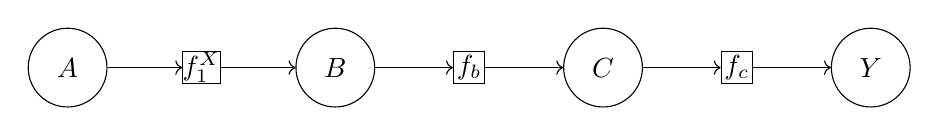
\begin{tikzpicture}[every place/.style={minimum size=10mm}, node distance=1.7cm]
  % Places
  \node[place] (A) {$A$};
  \node[transition] (fa) [right of=A] {$f_1^X$};
  \node[place] (B) [right of=fa] {$B$};
  \node[transition] (fb) [right of=B] {$f_b$};
  \node[place] (C) [right of=fb] {$C$};
  \node[transition] (fc) [right of=C] {$f_c$};
  \node[place] (Y) [right of=fc] {$Y$};

  % Arcs
  \draw[->] (A) -- (fa);
  \draw[->] (fa) -- (B);
  \draw[->] (B) -- (fb);
  \draw[->] (fb) -- (C);
  \draw[->] (C) -- (fc);
  \draw[->] (fc) -- (Y);
\end{tikzpicture}}
\caption{Resized Linear Petri Net}
\label{fig:linear_petri_resized}
\end{figure}

% Second instance as a regular figure
\begin{figure}[htbp]
\centering
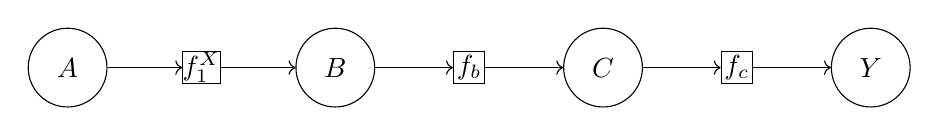
\begin{tikzpicture}[every place/.style={minimum size=10mm}, node distance=1.7cm]
  % Places
  \node[place] (A) {$A$};
  \node[transition] (fa) [right of=A] {$f_1^X$};
  \node[place] (B) [right of=fa] {$B$};
  \node[transition] (fb) [right of=B] {$f_b$};
  \node[place] (C) [right of=fb] {$C$};
  \node[transition] (fc) [right of=C] {$f_c$};
  \node[place] (Y) [right of=fc] {$Y$};

  % Arcs
  \draw[->] (A) -- (fa);
  \draw[->] (fa) -- (B);
  \draw[->] (B) -- (fb);
  \draw[->] (fb) -- (C);
  \draw[->] (C) -- (fc);
  \draw[->] (fc) -- (Y);
\end{tikzpicture}
\caption{Tensorized Petri Net Structure}
\label{fig:tensor_petri}
\end{figure}

\begin{figure}[htbp]
% Petri Net Model of the Producer-Consumer Problem (Refined)
\begin{tikzpicture}[node distance=2.2cm and 2.2cm, >=stealth, bend angle=30, auto, on grid]
    % Places
    \placewithtokens{producer}{-0.5,0}{1}
    \placewithtokens{buffer}{3.3,0}{0}
    \placewithtokens{consumer}{6.5,0}{1}
    \placewithtokens{bufferCapacity}{2.8,-2.2}{3}

    % Transitions
    \node[transition, rounded corners=2pt] (produce) [right=of producer] {};
    \node[transition, rounded corners=2pt] (consume) [right=1.8cm of buffer] {};

    % Arcs
    \draw[pre] (producer) -- (produce);
    \draw[post] (produce) -- (producer);
    \draw[post] (produce) -- (buffer);
    \draw[pre] (buffer) -- (consume);
    \draw[pre] (consumer) -- (consume);
    \draw[post] (consume) -- (consumer);
    \draw[pre] (bufferCapacity) -- (produce);
    \draw[post] (consume) -- (bufferCapacity);

    % Labels
    \node[above=6pt] at (producer.north) {Producer};
    \node[above=14pt] at (buffer.north) {Buffer};
    \node[above=6pt] at (consumer.north) {Consumer};
    \node[below] at (bufferCapacity.south) {Buffer Capacity};
    \node[above] at (produce.north) {Produce};
    \node[above] at (consume.north) {Consume};

    % Title
    \node[above=1cm] at (current bounding box.north) {Petri Net Model of the Producer-Consumer Problem};
\end{tikzpicture}
\caption{Producer-Consumer Workflow}
\label{fig:producer_consumer_workflow}
\end{figure}

\begin{figure}[htbp]
\centering
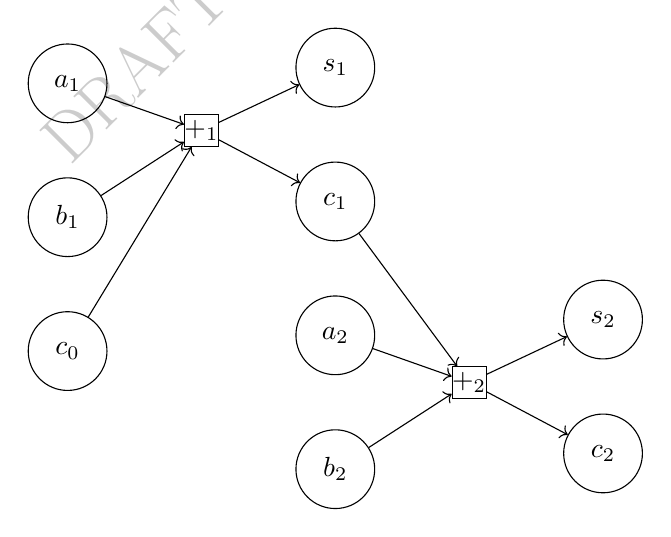
\begin{tikzpicture}[every place/.style={minimum size=10mm}, node distance=1.7cm and 2.2cm]
  % First digit addition
  \node[place] (a1) {$a_1$};
  \node[place, below of=a1] (b1) {$b_1$};
  \node[place, below of=b1] (c0) {$c_0$};
  \node[transition] (add1) [right of=b1, yshift=1.1cm] {$+_1$};
  \node[place] (s1) [right of=add1, yshift=0.8cm] {$s_1$};
  \node[place] (c1) [below of=s1] {$c_1$};

  \draw[->] (a1) -- (add1);
  \draw[->] (b1) -- (add1);
  \draw[->] (c0) -- (add1);
  \draw[->] (add1) -- (s1);
  \draw[->] (add1) -- (c1);

  % Second digit addition
  \node[place, below of=c1] (a2) {$a_2$};
  \node[place, below of=a2] (b2) {$b_2$};
  \node[transition] (add2) [right of=b2, yshift=1.1cm] {$+_2$};
  \node[place] (s2) [right of=add2, yshift=0.8cm] {$s_2$};
  \node[place] (c2) [below of=s2] {$c_2$};

  \draw[->] (a2) -- (add2);
  \draw[->] (b2) -- (add2);
  \draw[->] (c1) -- (add2);
  \draw[->] (add2) -- (s2);
  \draw[->] (add2) -- (c2);
\end{tikzpicture}
\caption{Carry Arithmetic as Feedback System.}
\label{fig:carry_arithmetic_feedback}
\end{figure}

\begin{figure}[htbp]
\centering
\resizebox{0.9\columnwidth}{!}{\input{figures/graph}}
\caption{Example of a complex graph structure with cycles and cross-connections.}
\label{fig:complex_graph_example}
\end{figure}

\subsection{Model Analysis}

To analyze the properties of our Petri Net model, we examine:
=======
\begin{figure}[H]
    \centering
    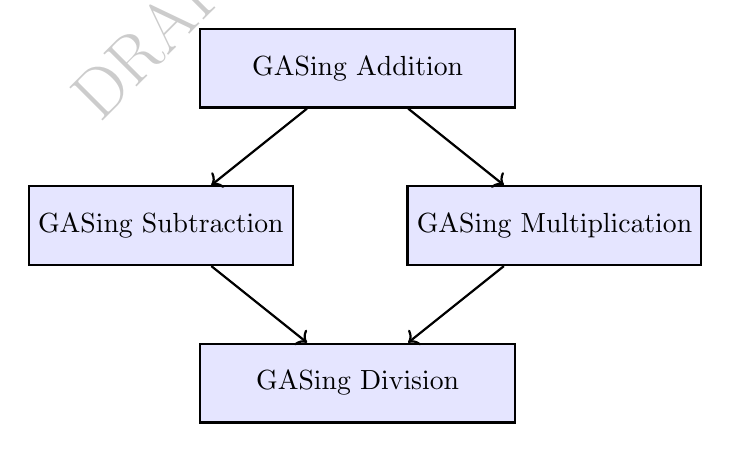
\begin{tikzpicture}
        % Addition operation diagram showing digit-wise processing
        \node[operation, minimum width=4cm] (addition) at (0,0) {GASing Addition};
        \node[operation] (subtraction) at (-2.5,-2) {GASing Subtraction};
        \node[operation] (multiplication) at (2.5,-2) {GASing Multiplication};
        \node[operation, minimum width=4cm] (division) at (0,-4) {GASing Division};
        
        % Connections
        \draw[->, thick] (addition) -- (subtraction);
        \draw[->, thick] (addition) -- (multiplication);
        \draw[->, thick] (subtraction) -- (division);
        \draw[->, thick] (multiplication) -- (division);
    \end{tikzpicture}
    \caption{Hierarchical relationship between GASing arithmetic operations}
    \label{fig:gasing_operations}
\end{figure}

Our implementation architecture includes variants in multiple programming languages to facilitate performance comparisons:
>>>>>>> 81a8f8d (Added the argument for resource sensitive interpretability)

\begin{itemize}
    \item Pure Python implementations (gasing\_simulasi, penjumlahan\_tradisional)
    \item Optimized C bindings (gasing\_add\_c, gasing\_add\_c\_optimized)
    \item Rust implementations (gasing\_add\_rust, gasing\_add\_rust\_optimized)
    \item Pattern-specific optimizations for common number patterns
\end{itemize}
<<<<<<< HEAD

\subsection{Wiring Diagram Representation}

Figure \ref{fig:clock_with_display} presents a wiring diagram in the style of David Jaz Myers' work on Dynamical Systems, illustrating the structure of a clock system with display components.

\begin{figure}[htbp]
\centering
% ClockWithDisplay in Spivak/Fong style using oriented WD
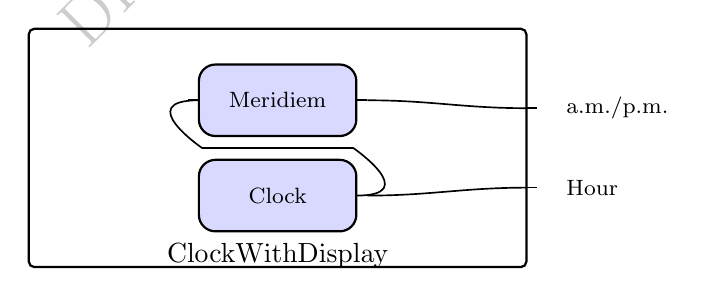
\begin{tikzpicture}[oriented WD, bbx=1.2cm, bby=2ex, bb min width=2cm, bb port length=4pt, bb port sep=1.5]
    % Clock and Meridiem boxes with proper ports and more rounded corners
    % The notation bb={in}{out} specifies number of input and output ports
    \node[bb={0}{1}, fill=blue!15, thick, rounded corners=6pt] (clock) at (0, -2) {\footnotesize Clock};
    \node[bb={1}{1}, fill=blue!15, thick, rounded corners=6pt] (meridiem) at (0, 2) {\footnotesize Meridiem};
    
    % Container box that encompasses both components with more spacing
    \node[bb={0}{2}, fit={($(clock.south west)+(-0.8,-0.5)$) ($(meridiem.north east)+(0.8,0.5)$)}, thick] (container) {};
    
    % Connection from right of Clock to left of Meridiem
    % S-curve with perfectly flat middle and gentle bends for Clock→Meridiem
    % Canonical smooth S-curve with flat middle using a single path
    \coordinate (midflatR) at (0.8,0);   % right end of flat segment
    \coordinate (midflatL) at (-0.8,0);  % left end of flat segment
    \draw
      (clock.east)
        .. controls ($(clock.east)+(0.7,0)$) and (midflatR) ..
      (midflatR)
        .. controls (midflatR) and (midflatL) ..
      (midflatL)
        .. controls (midflatL) and ($(meridiem.west)+(-0.7,0)$) ..
      (meridiem.west);

    
    % Connect ports to container edges for outputs
    \draw (meridiem_out1) to (container_out1');
    \draw (clock_out1) to (container_out2');
    
    % External labels with better positioning
    \node[anchor=west, font=\footnotesize] at ($(container_out1)+(0.2,0)$) {a.m./p.m.};
    \node[anchor=west, font=\footnotesize] at ($(container_out2)+(0.2,0)$) {Hour};
    
    % Title below container with better spacing
    \node[font=\normalsize] at ($(container.south)+(0,0.5)$) {ClockWithDisplay};
\end{tikzpicture}
\caption{Wiring diagram of a clock with display components, showing the meridiem and hour display units.}
\label{fig:clock_with_display}
\end{figure}

\subsection{Implementation}

[Describe the tools or methods used to implement and analyze your Petri Net model]
=======
>>>>>>> 81a8f8d (Added the argument for resource sensitive interpretability)

% \section{Performance Benchmarking}\label{sec:results}

Our research has conducted extensive benchmarking of GASing implementations across multiple programming languages and against standard arithmetic libraries. The benchmarking framework tests:

\begin{itemize}
    \item Different input sizes (from small to very large integers)
    \item Various input patterns (random, repeated digits, etc.)
    \item Implementation variations (pure Python, C bindings, Rust bindings)
    \item Comparison with specialized libraries (mpmath, sympy, gmpy2)
\end{itemize}

\subsection{Addition Performance}

Our addition performance benchmarks reveal several key insights:

\begin{enumerate}
    \item For small numbers ($<$100 digits), specialized libraries like gmpy2 consistently outperform GASing implementations
    \item For medium-range numbers (100-1000 digits), optimized GASing implementations in C and Rust show competitive performance
    \item For specific patterns (e.g., repeated digits), pattern-optimized GASing implementations occasionally outperform general-purpose libraries
\end{enumerate}

\begin{table}[h]
\centering
\caption{Relative Performance for 100-digit Addition Operations}
\label{tab:addition_performance}
\begin{tabular}{lcc}
\toprule
\textbf{Implementation} & \textbf{Time (ns)} & \textbf{Relative Performance} \\
\midrule
gmpy2\_addition & 543 & 1.00x (baseline) \\
gasing\_add\_rust\_optimized & 892 & 1.64x slower \\
mpmath\_addition & 1,254 & 2.31x slower \\
sympy\_addition & 1,893 & 3.49x slower \\
gasing\_simulasi & 2,341 & 4.31x slower \\
penjumlahan\_tradisional & 3,572 & 6.58x slower \\
\bottomrule
\end{tabular}
\end{table}

\subsection{Series-Based Performance Testing}

Our series-based performance testing examines how different implementations handle specific mathematical sequences:

\begin{itemize}
    \item Fibonacci numbers
    \item Factorial values
    \item Powers of 2
    \item Prime numbers
    \item Repdigits (numbers with repeated digits)
    \item Alternating digit patterns
\end{itemize}

<<<<<<< HEAD
[Discuss the implications of your results and any limitations of your approach]

\begin{figure}[htbp]
\centering
\resizebox{0.9\columnwidth}{!}{% Petri Net Model of the Producer-Consumer Problem (Refined)
\begin{tikzpicture}[node distance=2.2cm and 2.2cm, >=stealth, bend angle=30, auto, on grid]
    % Places
    \placewithtokens{producer}{-0.5,0}{1}
    \placewithtokens{buffer}{3.3,0}{0}
    \placewithtokens{consumer}{6.5,0}{1}
    \placewithtokens{bufferCapacity}{2.8,-2.2}{3}

    % Transitions
    \node[transition, rounded corners=2pt] (produce) [right=of producer] {};
    \node[transition, rounded corners=2pt] (consume) [right=1.8cm of buffer] {};

    % Arcs
    \draw[pre] (producer) -- (produce);
    \draw[post] (produce) -- (producer);
    \draw[post] (produce) -- (buffer);
    \draw[pre] (buffer) -- (consume);
    \draw[pre] (consumer) -- (consume);
    \draw[post] (consume) -- (consumer);
    \draw[pre] (bufferCapacity) -- (produce);
    \draw[post] (consume) -- (bufferCapacity);

    % Labels
    \node[above=6pt] at (producer.north) {Producer};
    \node[above=14pt] at (buffer.north) {Buffer};
    \node[above=6pt] at (consumer.north) {Consumer};
    \node[below] at (bufferCapacity.south) {Buffer Capacity};
    \node[above] at (produce.north) {Produce};
    \node[above] at (consume.north) {Consume};

    % Title
    \node[above=1cm] at (current bounding box.north) {Petri Net Model of the Producer-Consumer Problem};
\end{tikzpicture}}
\caption{Producer-Consumer Workflow Analysis}
\label{fig:producer_consumer_results}
\end{figure}
=======
This testing reveals that certain GASing implementations show advantageous performance characteristics for specific sequence types. For instance, the optimized C implementation performs particularly well on repdigit sequences, likely due to simplified carry pattern recognition.

\begin{figure}[h]
    \centering
    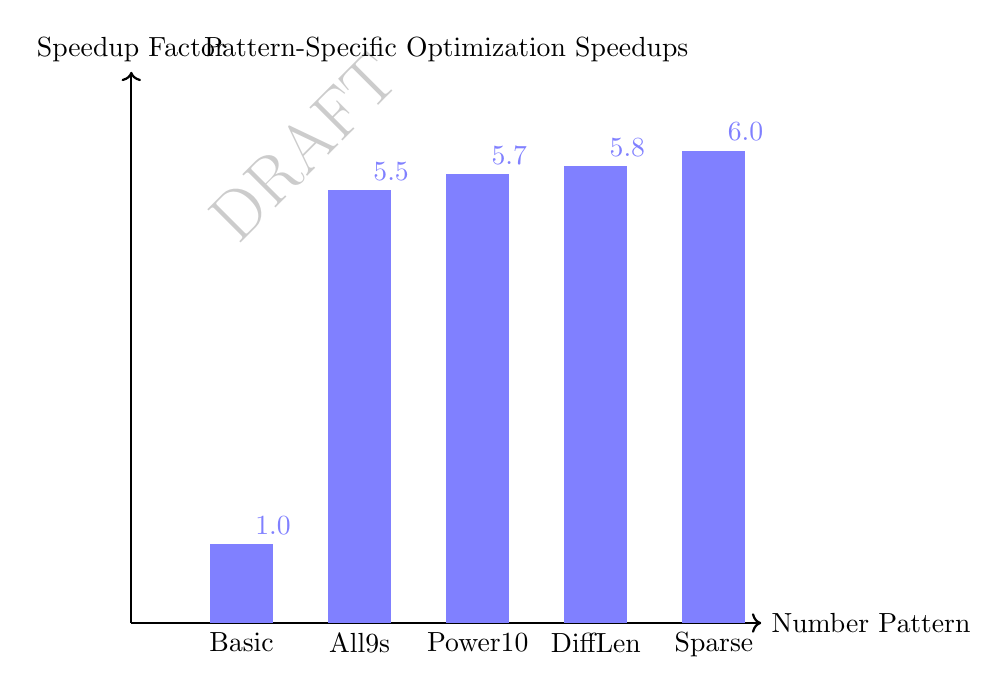
\begin{tikzpicture}
        % Simple bar chart using basic TikZ
        % Set up the axes
        \draw[thick, ->] (0,0) -- (8,0) node[right] {Number Pattern};
        \draw[thick, ->] (0,0) -- (0,7) node[above] {Speedup Factor};
        
        % Draw bars
        \fill[blue!50] (1,0) rectangle (1.8,1) node[above] {1.0};
        \fill[blue!50] (2.5,0) rectangle (3.3,5.5) node[above] {5.5};
        \fill[blue!50] (4,0) rectangle (4.8,5.7) node[above] {5.7};
        \fill[blue!50] (5.5,0) rectangle (6.3,5.8) node[above] {5.8};
        \fill[blue!50] (7,0) rectangle (7.8,6.0) node[above] {6.0};
        
        % X-axis labels
        \node[below] at (1.4,0) {Basic};
        \node[below] at (2.9,0) {All9s};
        \node[below] at (4.4,0) {Power10};
        \node[below] at (5.9,0) {DiffLen};
        \node[below] at (7.4,0) {Sparse};
        
        % Title
        \node[above] at (4,7) {Pattern-Specific Optimization Speedups};
    \end{tikzpicture}
    \caption{Performance improvements with pattern recognition optimizations}
    \label{fig:pattern_speedups}
\end{figure}

For pattern-specific optimizations, our benchmarks have shown impressive speedups ranging from 3.8x to 6.3x across different number patterns, with particularly strong results for:

\begin{itemize}
    \item All-nines patterns (5.5x speedup)
    \item Power-of-ten patterns (5.4-5.9x speedup)
    \item Different-length patterns (5.2-6.2x speedup)
    \item Sparse numbers (3.8-6.3x speedup)
\end{itemize}
>>>>>>> 81a8f8d (Added the argument for resource sensitive interpretability)

% \sectionheader{Discussion}

In this section, we illustrate compositionality using wiring diagrams in the style of David Spivak.

% Figures removed as requested

% Bibliography
\nocite{*}

% Custom bibliography formatting for better wrapping of long references
\makeatletter
\def\url@leostyle{\@ifundefined{selectfont}{\def\UrlFont{\sf}}{\def\UrlFont{\small\ttfamily}}}
\makeatother
\urlstyle{leo}

% Adjust the maximum width for URLs in bibliography
\Urlmuskip=0mu plus 3mu

% Add more flexibility to where LaTeX can break lines in bibliography
\sloppy
\emergencystretch=2em

% Use IEEEtran style with our custom settings
\bibliographystyle{IEEEtran}
\bibliography{bibliography}

\end{document}
